\documentclass[a4paper,10pt, twocolumn]{article}
\usepackage[utf8]{inputenc}
\usepackage{amsmath}
\usepackage{amssymb}
\usepackage{amsthm}
\usepackage[usenames,dvipsnames]{color}
\usepackage{comment}
\usepackage{tikz}
\usepackage{verbatim}
\usetikzlibrary{arrows,shapes}
\usepackage{listings}
\usepackage{algorithm}
\usepackage{algpseudocode}
\usepackage{hyperref}
\usepackage{graphicx}
\usepackage{epstopdf}
\usepackage{tabularx}
\usepackage{enumitem}
\setlist{nolistsep}
\setlength{\parindent}{0cm}

%page boarders
\usepackage[top=3cm, bottom=3cm, left=2cm, right=2cm]{geometry}
\usepackage[style=numeric,backend=bibtex]{biblatex}
\addbibresource{../sources}
%\usepackage[style=mla,babel=hyphen,backend=biber]{biblatex}

\tikzstyle{vertex}=[circle,fill=black!25,minimum size=20pt,inner sep=0pt]
\tikzstyle{edge} = [draw,thick,->,>=latex,shorten >=1pt]
\tikzstyle{weight} = [font=\small]
\tikzstyle{selected edge} = [draw,line width=2pt,->,red!75,>=latex]
\tikzstyle{residual edge} = [draw,thick,->,blue!75,>=latex]
\tikzstyle{vertexE}=[circle,fill=black!25,minimum size=20pt,inner sep=0pt]

% Declare layers (for more convenience when drawing graphs)
\pgfdeclarelayer{background}
\pgfsetlayers{background,main}

\newtheorem{lemma}{Lemma}
\newtheorem{corollary}[lemma]{Corollary}
%\newtheorem{proof}[lemma]{Proof}

\title{Parallel Network Flow Algorithms \\ 
\large A follow up seminar to the Parallel Algorithms lecture\footnote{Jesper Larsson Träff, lecture "Parallel Algorithms", 2012 winter term at TU Wien}}
\author{Martin Kalany, 0825673}

\begin{document}
\maketitle

\section{Abstract}
\label{sec:abstract}
We discuss the possibilities of parallelizing the problem of finding a maximum flow in a given flow network. Although intuitive sequential algorithms have been known for a long time, only in 1990 (TODO: check date) theoretical analysis of the problem was able to ascertain the inherently sequential nature of the problem\footnote{ assuming that $P \neq NP$.}, i.e., that no parallel algorithm that solves the problem in poly-logarithmic time with polynomially bounded resource consumption exists. Before this fundamental results, significant efforts were put into finding efficient parallel algorithms for this problem based on the PRAM model. We explain two fundamental results and compare them with later and improved developments.


\section{Introduction}
\label{sec:intro}
\emph{Maximum flow problem}\footnote{Henceforth called \lstinline|MAX-FLOW| for brevity}


\section{Network flows}
\label{sec:networkFlows}
A \textbf{flow network} \cite{ahuja93} is given by $N = (G,s,t,c)$, where
\begin{itemize}
	\item $G =(V,E)$ is a directed graph
    \item $s$ and $t$, $s \neq t$ are the source and terminal node
   	\item $c:E\rightarrow \mathbb{R}_0^{+}$ assigns a capacity $\forall a \in E$
   	\item $n=\lvert V\rvert$, $m=\lvert E\rvert$
\end{itemize}

Furthermore, the following assumptions are made:
\begin{itemize}
	\item $G$ is connected
	\item $G$ is simple, i.e., does not contain loops or parallel arcs
	\item $\nexists P(s,t)$ with infinite capacity
\end{itemize}

\medskip
$f:E \rightarrow \mathbb{R}_0^{+}$ is a \textbf{flow} if it satisfies:
\begin{itemize}
	\item \emph{Capacity constraints:} $f(e) \leq c(e)$ $\forall e \in E$
	\item \emph{Flow conservation:} 
	$ \sum\limits_{v \in V} f(u,v) =  0 \Leftrightarrow IN(f,v) = OUT(f,v)$ $\forall v \in V \setminus \{s,t\}$
	\item \emph{Skew symmetry:} $f(v,w) = -f(w,v)$
	\item \emph{Value of a flow:} $\lvert f\rvert = f(V,t)$ 
\end{itemize}

A flow $f$
\begin{itemize}
	\item is a \emph{maximum flow} if $\lvert f\rvert \geq \lvert f'\rvert$, for any other flow $f'$
	\item \emph{saturates} an arc e if $f(e) = c(e)$
	\item is a \emph{maximal (or blocking) flow} if every directed path P(s,t) contains at least one saturated arc
\end{itemize}
\medskip
The \emph{residual capacity} of $e \in V \times V$ w.r.t. a flow $f$ is defined as $c_r(e) = c(e) - f(e)$. $G_r = (V, E_r)$ is the \emph{residual network}, where $E_r = \left\{e \in V \times V \lvert c_r(e) > 0\right\}$. A path $P$ from $s$ to $t$ in $G_r$ is called an \emph{augmenting path} and can be used to increase the flow $f$.

\subsection{Algorithm of Ford-Fulkerson}
\label{sec:fordfulkerson}
The algorithm of Ford and Fulkerson \cite{ahuja93} is an intuitive sequential algorithm that solves \lstinline|MAX-FLOW|: starting from a null flow, increase the flow along an augmenting path as long as such a path exists. This is done by finding a path from $s$ to $t$ in the residual network along which the flow can be increased further. 

Figure \ref{fig:fordfulkerson1} depicts the flow network for which \lstinline|MAX-FLOW| is to be solved and an augmenting path\footnote{The residual network is equal to the given network in the first step.}. Note that this path may be chosen arbitrarily. Figure \ref{fig:fordfulkerson2} shows the residual network resulting from the situation in Figure \ref{fig:fordfulkerson1} and the next augmenting path. 

Note that this algorithm is restricted to integer capacities:  $c:E\rightarrow \mathbb{N}_0^{+}$ $\forall a \in E$. For a more detailed explanation and theoretical analysis, refer to \cite{ahuja93}.

\begin{figure}
\begin{center}
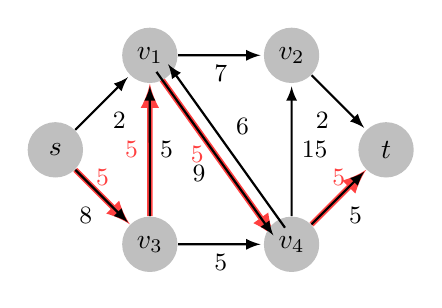
\begin{tikzpicture}[scale=1.2, auto,swap]
    % draw the vertices
	\foreach \pos/\name in {{(0,2)/s}, {(1,3)/v_1}, {(2.5,3)/v_2},
   	                        {(1,1)/v_3}, {(2.5,1)/v_4}, {(3.5,2)/t}}
    \node[vertex] (\name) at \pos {$\name$};
   	% Connect vertices with edges and draw weights
   	\foreach \source/ \dest /\weight in {s/v_1/2, s/v_3/8,v_3/v_1/5,
                                         v_1/v_2/7, v_4/v_2/15, v_3/v_4/5,
                                         v_2/t/2, v_4/t/5}
       	\path[edge] (\source) -- node[weight] {$\weight$} (\dest);
        	
       	%v_1/v_4/9
       	\path[edge] ([xshift= -2pt, yshift= 5pt] v_4.center) -- node[weight] {6}  ([xshift= 5pt, yshift= -2pt] v_1.center);
       	\path[edge] ([xshift = 2pt, yshift= -5pt] v_1.center) -- node[weight] {9}  ([xshift= -5pt, yshift= 2pt] v_4.center);
  
	% For convenience we use a background layer to highlight edges
   	% This way we don't have to worry about the highlighting covering
	% weight labels. 
	\begin{pgfonlayer}{background}
   	    \foreach \source /\dest  /\weight in {s/v_3/5,v_4/t/5}
	        \path[selected edge] (\source) -- node[weight,above] {$\weight$}(\dest);		
            \path[selected edge] ([xshift = 2pt, yshift= -5pt] v_1.center) -- node[weight,left] {5}  ([xshift= -5pt, yshift= 2pt] v_4.center);
            \path[selected edge] (v_3) -- node[weight,left] {$5$}(v_1);
   	\end{pgfonlayer}
\end{tikzpicture}
\end{center}
\caption{Algorithm of Ford-Fulkerson: Initial network (black) and first augmenting path (red)}
\label{fig:fordfulkerson1}
\end{figure}

\begin{figure}
\begin{center}
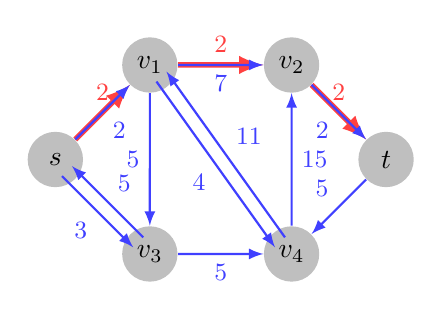
\begin{tikzpicture}[scale=1.2, auto,swap]
   	% draw the vertices
    \foreach \pos/\name in {{(0,2)/s}, {(1,3)/v_1}, {(2.5,3)/v_2},
    	                        {(1,1)/v_3}, {(2.5,1)/v_4}, {(3.5,2)/t}}
    \node[vertex] (\name) at \pos {$\name$};
   	% Connect vertices with edges and draw weights
   	\foreach \source/ \dest /\weight in {s/v_1/2, v_1/v_3/5, t/v_4/5,
                                         v_1/v_2/7, v_4/v_2/15, v_3/v_4/5,
                                         v_2/t/2}
       	\path[residual edge] (\source) -- node[weight] {$\weight$} (\dest);

        	%s/v_3/8,
       	\path[residual edge] ([xshift= -2pt, yshift= 5pt] v_3.center) -- node[weight] {5}  ([xshift= 5pt, yshift= -2pt] s.center);
       	\path[residual edge] ([xshift = 2pt, yshift= -5pt] s.center) -- node[weight] {3}  ([xshift= -5pt, yshift= 2pt] v_3.center);
        	%v_1/v_4/9
       	\path[residual edge] ([xshift= -2pt, yshift= 5pt] v_4.center) -- node[weight] {11}  ([xshift= 5pt, yshift= -2pt] v_1.center);
       	\path[residual edge] ([xshift = 2pt, yshift= -5pt] v_1.center) -- node[weight] {4}  ([xshift= -5pt, yshift= 2pt] v_4.center);       	
        	
       	\begin{pgfonlayer}{background}
   	    \foreach \source /\dest  /\weight in {s/v_1/2,v_1/v_2/2,v_2/t/2}
            \path[selected edge] (\source) -- node[weight,above] {$\weight$}(\dest);			            
   	\end{pgfonlayer}
\end{tikzpicture}
\end{center}
\caption{Algorithm of Ford-Fulkerson: Residual network (blue) and augmenting path (red)}
\label{fig:fordfulkerson2}
\end{figure}	




\section{Model of Computation}
\label{sec:model}
We use the \textbf{PRAM} Model\footnote{Parallel Random Access Machine} as the model of computation. Specifically, a \textbf{MIMD} - Multiple Instructions Multiple Data - variant is used, where each processor $p$ executes a distinct set of instructions on distinct data. Instructions are executed in lock-step and any necessary padding of instructions is assumed to be done automatically. 

\section{Computitional Complexity}
\label{sec:cc}
The algorithmic complexity of the \emph{Ford-Fulkerson} algorithm is given as $O((n+m)*f_{max})$\footnote{$f_{max}$ is from here on used to denote the maximum flow} \cite{ahuja93,papa95}. This was improved by the \emph{Edmonds-Karp} algorithm to $O(n*m^2)$, by using shortest augmenting paths instead of arbitrarily chosen ones. Clearly, the \emph{maximum flow problem} can be solved in polynomial time with a sequential algorithm and is thus $\in P$.

Informally, algorithms may be \emph{efficiently parallelizeable} or \emph{inherently sequential}. The complexity class \textbf{NC} \cite{papa95} ("Nick's Class") contains all problems solvable in $O(log^{k_1}(n))$ time and $O(n^{k_2})$ total work. We give a useful alternate definition:  A language that is decided by PRAM in $O(log^{k_1}(n))$ time steps with $O(n^{k_2})$ processors available at each step is in $NC$. Problems $\in NC$ thus are solvable  in poly-logarithmic time requiring polynomial work (or resources). Problems $P \setminus NC$ are dubbed "inherently sequential", i.e., not parallelizeable efficiently. 

Clearly, $NC \subseteq P$, but whether $NC \subset P$ or $NC = P$ is still unknown. It follows that we do not know whether or not inherently sequential problems actually exist. The most likely problems to be hard to parallelize are P-complete problems. Since any problem $A \in P$ can be reduced to a P-complete problem $B$, a parallel algorithm that solves $B$ within poly-logarithmic time bounds would immediately imply that for all problems $\in P$ a parallel algorithm $\in NC$ exists \cite{papa95}.

As an example, the Ford-Fulkerson algorithm can not be parallelized trivially. Although constructing the residual network can be done in constant time $O(1)$ by assigning a processor to each edge $a \in E$ and augmenting paths can be found in $O(log^{2}n)$ time and $O(n^{2})$ work by a basic BFS search, the number of stages can not be reduced to less than $O(\sqrt(n))$ \cite{ahuja93}. Thus the total complexity, which is dominated by the number of stages, places the algorithm in $P \setminus NC$.
	
As shown in \cite{papa95}, \lstinline|MAX-FLOW| is P-complete and no parallel algorithm $\in NC$ is currently known for solving this problem. It is assumed that the problem is inherently sequential.

\section{Dinitz' scheme}
\label{sec:dinitz}
$N = (V,E,s,t,c)$ is a \textbf{layered network} \cite{yossi81} if each vertex $v \in V$ has a layer number $l(v)$ s.t.
\begin{itemize}
	\item $l(s) = 0$ and $0 \leq l(v) \leq l(t)$ $\forall v \in V$
	\item $(e = u \rightarrow v) \in E  \Rightarrow l(v) - l(u) = 1$
\end{itemize}
Figure \ref{fig:dinitz} shows a layered network and it's underlying directed acyclic network.

\begin{figure}
\begin{center}
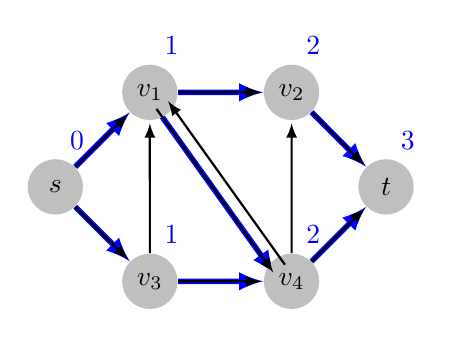
\begin{tikzpicture}[scale=1.2, auto,swap]
   	% draw the vertices
	\foreach \pos/\name/\layer in {{(0,2)/s/0}, {(1,3)/v_1/1}, {(2.5,3)/v_2/2},
    	                        {(1,1)/v_3/1}, {(2.5,1)/v_4/2}, {(3.5,2)/t/3}}
    \node[vertex,label={[color=blue]80:$\layer$}] (\name) at \pos {$\name$};
        
    %\node[vertex,label={[color=blue]80:$+12$}] (v_1) at (1.5,3) {$v_1$};
    % Connect vertices with edges and draw weights
    \foreach \source/ \dest in {s/v_1, s/v_3,v_3/v_1,
                                        v_1/v_2, v_4/v_2, v_3/v_4,
                                        v_2/t, v_4/t}
     \path[edge] (\source) -- (\dest);
        	
     %v_1/v_4/9
     \path[edge] ([xshift= -2pt, yshift= 5pt] v_4.center) -- ([xshift= 5pt, yshift= -2pt] v_1.center);
     \path[edge] ([xshift = 2pt, yshift= -5pt] v_1.center) -- ([xshift= -5pt, yshift= 2pt] v_4.center);
  
	% For convenience we use a background layer to highlight edges
    % This way we don't have to worry about the highlighting covering
	% weight labels. 
	\begin{pgfonlayer}{background}
    	\foreach \source /\dest in {s/v_3,v_2/t,s/v_1,v_1/v_2,v_3/v_4,v_4/t}
	      	\path[selected edge, color=blue] (\source) -- (\dest);		
	    \path[selected edge, color=blue] ([xshift = 2pt, yshift= -5pt] v_1.center) -- ([xshift= -5pt, yshift= 2pt] v_4.center);
	\end{pgfonlayer}
\end{tikzpicture}
\end{center}
\caption{A layered network (in blue) with layer numbers and it's underlying network}
\label{fig:dinitz}
\end{figure}

\begin{corollary}
\textbf{Dinitz' scheme} \cite{dinitz70} \\
A maximum flow problem in a general network can be transformed into $O(n)$ maximal flow problems in layered networks.
\end{corollary}

A layered network can easily be constructed from a directed acyclic network by performing breath-first search in  $O(log^{2}n)$ time. It follows that an algorithm that finds a maximal/blocking flow in a layered network can solve \lstinline|MAX-FLOW| in $O(n)$ iterations. The basic scheme is given in Algorithm \ref{algo:dinitz}

%TODO: remove comments?
\begin{algorithm}
\caption{Dinitz' scheme}
\label{algo:dinitz}
\begin{algorithmic}[1]
	\Function{MAX-FLOW}{$N=(V,E,s,t,c)$}
	\State start with some valid flow 
	\While{$l(t) \neq \infty$} \Comment{\textcolor{OliveGreen}{$O(n)$}}	
		\State Construct residual network $G_r$ \Comment{\textcolor{OliveGreen}{$O(n)$, $p=O(n)$}}
		\State Construct layered network $G_l$ from $G_r$ \Comment{\textcolor{OliveGreen}}{$O(m/p + n)$}
		\State $f_l$ = MAX-FLOW($G_l$)  \Comment{tbd}
		\State $f$ = $f$ + $f_l$ \Comment{\textcolor{OliveGreen}{$O(n)$}}
	\EndWhile
	\EndFunction
\end{algorithmic}
\end{algorithm}

\section{Algorithm of Shiloach and Vishkin}
\label{sec:shiloach}
The Shiloach-Vishkin algorithm is based on Dinitz' scheme as shown in Section \ref{sec:dinitz}. This section focuses on the implementation of an algorithm to solve \lstinline|MAX-FLOW| for a given layered network.

The following notation will be used:
\begin{itemize}
	\item \lstinline|EXCESS(v)|: The amount of excessive flow at node $v$. \lstinline|EXCESS(v)| = $IN(f,v) - OUT(f,v) \geq 0$.
	\item \lstinline|UNBALANCED|: The set of vertices that hold some excess flow. \lstinline|UNBALANCED| = $\{v \in V \lvert EXCESS(v) > 0 \}$. The implementation uses a queue to maintain FIFO order on the set of unbalanced vertices.
	\item \lstinline|blocked|: A vertex v is blocked if for all it's outgoing edges $e_i = (v, u_i)$, $e_i$ is either saturated or $u_i$ is blocked\footnote{The sink vertex $t$ is never blocked}. 
\end{itemize}

The algorithm operates in \emph{pulses}: In the first pulse, all outgoing edges of $s$ or saturated: $\forall e_i = (s, v_i):$ $f(e_i) = c(e_i)$. The set of unbalanced vertices at the end of pulse 1 is thus the set of all neighbours of $s$: \lstinline|UNBALANCED| = $\{v_i\lvert \exists (s, v_i) \in E \}$. In each subsequent pulse, the unbalanced vertices try to push forward\footnote{i.e., to the next layer of the network} as much of their excessive flow as possible. Any remaining excessive flow will be returned backward. All balanced vertices remain idle during the pulses. The algorithm terminates as soon as no unbalanced vertices are available, implying that all flow reach the source $s$ or sink $t$.

Algorithm \ref{algo:sv} shows the routine for solving \lstinline|MAX-FLOW| in a given layered network. Functions \lstinline|PUSH| and \lstinline|RETURN| are depicted in Algorithm \ref{algo:sv_push} and Algorithm \ref{algo:sv_return}, respectively and will be explained in detail in the remainder of this section. The algorithm maintains the number of the current pulse in $i$.

\begin{algorithm}
\caption{Shiloach-Vishkin}
\label{algo:sv}
\begin{algorithmic}[1]
	\Function{MAX-FLOW}{$G_l$}
		\State EXCESS(s) = $\Sigma_{v \in L_1}$ c(s$\rightarrow$v)
		\State PUSH(s, EXCESS(s))
		i = 1;
		\While{$\exists$ v $\in$ UNBALANCED}
			\State i++
			\ForAll {$v \in UNBALANVED$}			
				\If{$v$ is not blocked}
					\State PUSH(v, EXCESS(v))
				\EndIf
			\EndFor
			\State RETURN(v, EXCESS(v))
		\EndWhile
	\EndFunction
\end{algorithmic}
\end{algorithm}

\subsection{Partial Sums trees}
\label{sec:sv_pstrees}
A \emph{partial sums tree}\footnote{Abbreviated PS-tree from here on.} is a complete binary tree with the leftmost $k$ leaves associated with $k$ numbers $a_1,...,a_k$. A partial sums tree is of height $h = \lceil log_2(k) \rceil$ and has $w = 2^{\lceil log_2(k) \rceil}$ leaves. The remaining $w - k$ rightmost leaves are associated with 0. Each internal node of a partial sums tree stores the sum of it's child nodes. Thus, the root node stores the sum of all leaves of the tree. Figure \ref{fig:pstree} provides an example.

\begin{figure}[H]
\begin{center}
  \begin{tikzpicture}[scale=0.8,label distance=-3mm,>= latex, node distance = 2cm,level/.style={sibling distance=40mm/#1}]
    \tikzstyle{every node}=[draw=none,fill=none, minimum size=5mm,font=\footnotesize];

   \node (pr) {$23$}
   	child {node (p13) {$17$}
	  	child {node (p9) {$8$} 
    	 	child {node (p1) {$5$}}
      		child {node (p2) {$3$}}
    		}
  		child {node (p10) {$9$} 
    	  	child {node (p3) {$2$}}
      		child {node (p4) {$7$}}
   		 }
   	}
   	child {node (p14) {$6$} 
   		child {node (p11) {$6$} 
      		child {node (p5) {$6$}}
		    child {node (p6) {$0$}}
    		}
   		child {node (p12) {$0$} 
      		child {node (p7) {$0$}}
      		child {node (p8) {$0$}}
      	}
    };
\end{tikzpicture}
\end{center}
\caption{A partial sums tree with $k=5$}
\label{fig:pstree}
\end{figure}

A \emph{flow quantum} is a 3-tuple $(p, e, f)$, where $p$ is the number of the pulse during which some flow of value $f$ reached a vertex $v$ via edge $e$.

For the parallel implementation of \lstinline|PUSH| and \lstinline|RETURN|, several PS-trees will be used. Four PS-trees are attached to every vertex $v \in V$:
\begin{itemize}
	\item T-OUT(v): Each active leave $a_i$ is associated with an outgoing edge $e_i = (v, w_i)$. $a_i = c(e_i) - f(e_i)$ ,i.e., $a_i$ stores the residual capacity of $e_i$. T-OUT(v) has $d_{out}(v)$\footnote{As usual, $d_{in}(v)$ and $d_{out}(v)$ designate the in- and out-degree of a vertex} active leaves.
	\item T-IN(v): Records flow quanta reaching $v$. T-IN(v) has $2n*d_{in}(v)$ active leaves to be able to record the pulse\footnote{As shown in Section \ref{sec:sv_analysis}, the number of pulses is bounded by $O(2n)$} and edge for each flow quantum that reaches $v$. 
	\item T-ACCESS(v): Each of the $d_{in}(v)$ active leaves is associated with one edge entering $v$. Used to coordinate access to $v$.
	\item T-SUM(v): Sums up the flow returned to $v$ in a given pulse. $d_{out}(v)$ active leaves. 
\end{itemize}
One PS-tree is attached to every arc $e \in E$:
\begin{itemize}
	\item T-EDGE(v): $2n$ active leaves, each of which is associated with one pulse to record the amount of flow returned on $e$ in a given pulse.
\end{itemize}

Let T be a PS-tree. Every node of T is represented by $T[height, i]$, where $height(root) = \lceil log_2(k) \rceil$ and $heigt(a_i) = 1$ , $\forall$ leaves $a_i$. Additionally, $T[root]$ designates the root node of T. We define the following operations on T:
\begin{itemize}
	\item CLEAR(i): The value of all nodes on the path $P(T[1,i],root)$ is set to 0. Note that executing this operation for less than all leaves will result in an invalid PS-tree. When executing the operation for all leaves, several processes will attempt to write to the same node. Thus a CRCW-PRAM is required.
%TODO: more detailed explaination of required PRAM
	\item UPDATE(i,$a_i$): The value of the $i^{th}$ leave is set to $a_i$ and the values of all nodes on the path $P(T[1,i],root)$ are updated.
	\item SUM(i, $S_i$): Calculate the sum of leave nodes up to $a_i$. $S_i = a_1,...,a_i$.
	\item FIND($\alpha$, k, $\rho$): Given $\alpha$, find $k$ and $\rho$ s.t. $a_1+...+a_{k-1} < \alpha \leq a_1+...+a_k$ and $\rho = \alpha - (a_1+...+a_{k-1}$.
\end{itemize}  

\subsection{Parallel Implementation}
\label{sec:sv_parImpl}
We use the following processor assignment:
\begin{itemize}
	\item Each vertex $v \in V$ has a processor $P(v)$ assigned
	\item Each edge $e \in E$ has a processor $P(e)$ assigned
	\item Each flow quantum $Q$ has a processor $P(Q)$ assigned. In other words, each leaf in each of the $2n * d_{in}(v)$ T-IN(v) PS-trees has a processor $P(Q)$ assigned.
\end{itemize}

The following lemma states that the apparently large number of required processors can be reduced to $n$. However, the above assignment is useful for a clear presentation of the algorithms.

\begin{lemma}
An allocation of processors to jobs s.t. $n$ processors are sufficient is possible. 
\end{lemma}

\begin{proof}
%TODO
TODO
\end{proof}

In addition to the four PS-trees attached to each vertex $v$, $v$ keeps two pointers:
\begin{itemize}
	\item head(v): Points to the rightmost significant leave in T-in($v$). The rightmost significant (i.e., the rightmost leave with a value $\neq 0$) is associated with the flow quanta that was the last to reach $v$. head(v) will be used to return excess flow. 
	\item $k'$: The outgoing edges of $v$ are assumed to be ordered arbitrarily. $k'$ points to the first outgoing edge\footnote{the edge with the smallest index w.r.t. the given ordering} that is not yet saturated. In other words, $k'$ points to the next edge that can be utilized to push excess flow from $v$.  
\end{itemize}

In Algorithms \ref{algo:sv_init}, \ref{algo:sv_push} and \ref{algo:sv_return}, the notation \textcolor{blue}{P():} is used to indicate that the following instructions are carried out only by the specified processors. Algorithm \ref{algo:sv_init} shows the initialization routine executed at the beginning of each pulse. Each processor assigned to an edge $e_j = (v, w)$ updates the PS-tree T-OUT attached to $v$ s.t. it's leave $a_j$ is assigned the residual capacity of $e_j$. $f(e_j$) is set to 0. In the next step, each processor assigned to a vertex $v$ initializes it's pointers $head(v)$ and $k'(v)$.

\begin{algorithm}
\caption{Shiloach-Vishkin: INITIALIZE}
\label{algo:sv_init}
At beginning of each pulse:	
\begin{algorithmic}[1]
	\Function{INTIALIZE}{v}
		\State \textcolor{blue}{P($e_j = v \rightarrow w$):}
		\State UPDATE($j$, $c_r(e_j)$) T-OUT(v)
		\State f($e_j$) = 0
		\State \textcolor{blue}{P(v):}
		\State head(v) = 0	
		\State k'(v) = 1	
 	\EndFunction
\end{algorithmic}
\end{algorithm}

TODO: explain algorithms

\begin{algorithm}
\caption{Shiloach-Vishkin: PUSH}
\label{algo:sv_push}
$\forall v \in UNBALANCED$ do in parallel:
\begin{algorithmic}[1]
	\Function{PUSH}{v,EXCESS(v)}
		\State \textcolor{blue}{P(v):}
		\State $\alpha$ = min\{EXCESS(v), T-OUT(v)[root]\} 
		\State EXCESS(v) = EXCESS(v) - $\alpha$
		\State FIND($\alpha$, k, $\rho$) in T-OUT(v)
		\State \textcolor{blue}{P($e_j = v \rightarrow w$):}
		\If{k' $\leq$ j $\leq$ k}
 		\State UPDATE(j,1) in T-ACCESS(w)
		\State SUM(j,$S_j$) in T-ACCESS(w)
		\If{$j == k$}
			$q_j$ = $\rho$
		\Else
			\State $q_j$ = T-OUT(v)[1,j]
		\EndIf
		\State $f(e_j)$ = $f(e_j)$ + $q_j$
		\State TOTAL(w) = T-IN(w)[root]
		\State UPDATE(head(w) + $S_j$, $q_j$) in T-IN(w)
		\State UPDATE(j, T-OUT(v)[1,j] - $q_j$) in T-OUT(v)
		\State head(w) = head(w) + T-ACCESS(w)[root] 
		\State CLEAR(j) in T-ACCESS(w)
		\State EXCESS(w) = T-IN(w)[root] - TOTAL(w)
		\EndIf
		\State \textcolor{blue}{P(v):} k' = k
		\State \textcolor{blue}{P($e_d = v \rightarrow w$):}
		\If{EXCESS(v) $>$ 0}
			\State block v
		\EndIf
 	\EndFunction
\end{algorithmic}
\end{algorithm}


\begin{algorithm}
\caption{Shiloach-Vishkin: RETURN}
\label{algo:sv_return}
\begin{algorithmic}[1]
	\Function{RETURN}{v, EXCESS(v)}
		\State \textcolor{blue}{P(v):}
		\State FIND (T-IN(v)[root] - EXCESS(v), k, $\rho$) in T-IN(v)
		\State EXCESS(v) = 0
		\State \textcolor{blue}{$P(Q_j = (e_j = u \rightarrow v, q_j))$:}
		\State $d_j \rightarrow q_j$ for $k < j \leq head(v)$
		\State $d_j \rightarrow q_j - \rho$ if $j = k$
		\State UPDATE(j, 0) in T-IN(v) for $k < j \leq head(v)$
		\State UPDATE(j, $\rho$) in T-IN(v) if $j = k$
		\State UPDATE($r_j$,$d_j$) in T-EDGE($e_j$)
		\State $f(e_j)$ = $f(e_j)$ - T-EDGE($e_j$)[root]
		\State UPDATE($l_j$, T-EDGE($e_j$)[root] in T-SUM(u)
		\State EXCESS(u) = EXCESS(u) + T-SUM(u)[root]
		\State CLEAR($r_j$) in T-EDGE($e_j$)
		\State CLEAR($l_j$) in T-SUM(u)
		\State \textcolor{blue}{P(v):}
		\State head(v) = k
	\EndFunction
\end{algorithmic}
\end{algorithm}

\subsection{Analysis}
\label{sec:sv_analysis}
The comments in Algorithm \ref{algo:dinitz} state the complexity of the steps: According to Dinitz' scheme, the while-loop is bounded by $O(n)$ iterations. Constructing the residual network $G_r$ can trivially be done in $O(n)$ using n processors, since $m = O(n^{2})$. Breath-first search can be used to construct a layered network $G_l$ out of $G_r$. Efficient parallel implementations of BFS run in $O(m/p +n)$ time using n processors. Adding the found \lstinline|MAX-FLOW| of a layered network to the global \lstinline|MAX-FlOW| can again be done in $O(n)$ time. It remains the calculate the complexity of finding a \lstinline|MAX-FlOW| in a layered network $G_l$, as shown in Algorithm \ref{algo:sv}.

Each \lstinline|PUSH| or \lstinline|RETURN| operation requires $O(log n)$ steps, since they do not contain any loops and statements operate on paths from a leave to the root of a binary tree of height $\lceil log_2(k) \rceil$.
\begin{lemma}
The number of pulses in each round is at most $2n$
\end{lemma}
\begin{proof}
TODO
\end{proof}

It follows that each round is executed in $O(n*log n)$ time and thus the algorithm overall has a time complexity of $O(n^{2} * log n)$. As shown in Section \ref{sec:sv_pstrees}, a CRCW PRAM is required for the operations on PS-trees. However, Shiloach and Vishkin claim\cite{yossi81}, that a CREW PRAM is sufficient to execute the algorithm within the given bounds, since any concurrent write to a specific memory location will attempt to write the same value. Unfortunately, the paper does not substantiate this claim. 

\section{Algorithm of Goldberg and Tarjan}
\label{sec:goldberg}
The Goldberg-Tarjan algorithm solves \lstinline|MAX-FLOW| on directed acyclic graphs. Contrary to the Shiloach-Vishkin algorithm presented in Section \ref{sec:shiloach}, it is not based on Dinitz' scheme (see Section \ref{sec:dinitz}. The algorithm constructs a blocking flow by moving flow through the network while maintaining a blocking pre-flow. Intuitively, the flow quanta do a depth-first search from $s$ to $t$ in a dynamic graph, where edges become saturated and vertices become blocked.

An \textbf{atom} a is defined as the maximal quantity of flow that so far moved along the same path $P(s,v)$. An atom a can move along forwards on an edge $e \in E$, or backwards along the same edge. Formally, the backward edges are defined as $E^{-1} = \{(w,v)\vert (v,w) \in E \}$. Furthermore, an atom a has the following properties:
\begin{itemize}
	\item \textbf{size(a)}: the amount of excess flow that a carries.
	\item \textbf{position(a)}: the vertex $v \in V$ the atom is currently located at.
	\item \textbf{trace(a)}: The trace, i.e., the sequence of edges the atom a moved so far. $P_t(s, position(a))$ in $E \cup  E^{-1}$. 
	\item \textbf{path(a)}: The simple Path $P_s(s, position(a))$ in $E$. $(v,w) \in P_s$ if $(v,w) \in P_t \and (w,v) \not\in P_t$. In other words, if an atom a traversed an edge $(v,w)$ both forwards and backwards, $(v,w) \in P_t$ but $(v,w) \not\in P_s$.  
\end{itemize}

TODO: explain algorithms

\begin{algorithm}
\caption{Goldberg-Tarjan: INITIALIZE}
\label{algo:gt_init}
\begin{algorithmic}[1]
	\Function{INITIALIZE}{$N=(V,E,s,t,c)$}
	\ForAll{$e_i = (s,v_i) \in E$}
		\State create new atom $a_i$
		\State $size(a_i) = c(e_i)$
		\State $position(a_i) = v_i$
		\State $trace(a_i) = (s,v_i)$		
	\EndFor
	\EndFunction
\end{algorithmic}
\end{algorithm}

\begin{algorithm}
\caption{Goldberg-Tarjan: PUSH}
\label{algo:gt_push}
$\forall v \in V \setminus \{s,t\}$ and $v$ not blocked, do in parallel:
\begin{algorithmic}[1]
	\Function{PUSH}{$v$}
	\State Let $a_1 \dots a_k$ be atoms at vertex $v$
	\State Let $(v,w_1) \dots (v,w_l)$ be admissible arcs at $v$
	\State $\forall 1 \leq j \leq k: S(j) = \Sigma_{i=1}^{j} size(a_i)$
	\State $\forall 1 \leq j \leq l: R(j) = \Sigma_{i=1}^{j} c_r(v,w_i)$
	\State Assign $a_i$ to $(v, w_j)$:
	\If {$S(i) - size(a_i) \geq R(j) - c_r(v, w_j)$}
		\If{$S(i) \leq R(j)$}
			\State assign amount $size(a_i)$ of $a_i$ to $(v,w_j)$
		\Else
			\State assign amount $R(j)-S(i)+size(a_i)$ of $a_i$ to $(v,w_j)$
		\EndIf
	\EndIf
	\If {$S(i) - size(a_i) < R(j) - c_r(v, w_j)$}
		\If{$S(i) > R(j)$}
			\State assign amount $c_r(v,w_j)$ of $a_i$ to $(v,w_j)$
		\Else
			\State assign amount $S(i)-R(j)+c_r(v,w_j)$ of $a_i$ to $(v,w_j)$
		\EndIf
	\EndIf
	\If{$a_i$ assigned to more than 1 $(v,w_j)}$
		\ForAll{$(v,w_j)$ assigned to $a_i$}
			\If{assignment saturates $(v,w_j)$}
				\State create new atom $a_k$ 
				\State $size(a_k$) = quanta assigned to $(v,w_j)$
				\State $trace(a_k) = trace(a_i)$ 
				\State $position(a_k) = position(a_i)$
			\EndIf
		\EndFor
	\EndIf	
	\ForAll{$(v,w_j)$}
		\ForAll{$a_i \leftrightarrow (v,w_j)$}
			\State $f(v,w_j) = f(v,w_j) + size(a_i)$
			\State $location(a_i) = w_j$
			\State $trace(a_i) = trace(a_i) + w_j$
		\EndFor 
	\EndFor
	\If{$\forall (v,w_j):$ saturated}
		\State mark $v$ to block
	\EndIf	
	\State $\forall v_i$ marked to block: $block(v_i)$
	\ForAll{$w \in V$ and $w$ blocked}
		\ForAll{$a$ at $w$}
			\State Let $(v_a, w)$ be last arc on $trace(a)$
			\State $f(v_a, w) = f(v_a, w) - size(a)$
			\State $location(a) = v_a$
			\State $trace(a) = trace(a) - (v_a, w)$
		\EndFor
	\EndFor	
	\EndFunction
\end{algorithmic}
\bigskip
Repeat PUSH until all atoms arrive at $s$ or $t$
\end{algorithm}

\subsection{Correctness}
\label{sec:gt_correctness}
The following observations are important for the analysis of the algorithm:
\begin{itemize}
	\item Atoms can move forward on an edge $e=(v,w) \in E$, increasing the flow $f(v,w)$.
	\item or backward on $e^{-1}=(w,v)$, decreasing $f(v,w)$ and blocking $w$. 
	\item The flow along an edge $f(v,w)$ never becomes negative: an atom can only move backward on $e^{-1}=(w,v)$ if it moved along $e=(v,w)$ first.
	\item $f(v,w)$ increases until $w$ is blocked, after which $f(v,w)$ decreases.
\end{itemize}

TODO: proof correctness


\subsection{Analysis}
\label{sec:gt_analysis}
\begin{lemma}
The number of created atoms is $\leq m$.
\end{lemma}
\begin{proof}
Atoms created in algorithm
\begin{itemize}
	\item INITIALIZE: $\lvert (s,v_i) \in E \rvert$. $size(a_i) = c(s,v_i)$
	\item PUSH: Splitting an atom: The newly created atom $a'$: $size(a') = c_r(v,w)$ is assigned the residual capacity of an edge $(v,w)$.
\end{itemize}
Clearly, each newly created atom in \lstinline|INITIALIZE| and \lstinline|PUSH| saturates an arc. Each arc may be saturated only once, which implies the claim.
\end{proof}

\begin{lemma}
$\forall a_i:$ at any time, $\lvert trace(a_i) \rvert \leq 2n-3$ arcs.
\end{lemma}
\begin{proof}
\item An atom $a_i$ only moves backwards on $(v,w) \in E$ once $w$ is blocked. Since $a_i$ moved forwards and backwards on $(v,w)$, $w \notin P_s(a_i)$. $a_i$ never visits $w$ again, since $w$ is now blocked. This implies the following two statements about $trace(a_i$):
\begin{itemize}
	\item $\forall w \in V \setminus \{t\}: trace(a_i)$ contains $(v,w)$ at most once, since an atom $a_i$ may traverse an arc in forward direction at most once. Any arc $(w,t)$ can not be on the trace. Otherwise $a_i$ would have reached the sink node $t$.
	\item $\forall w \in V \setminus \{s,t\}: trace(a_i)$ contains $(w,v)$ at most once, since an atom $a_i$ may traverse an arc in backward direction at most once. Any arc $(t,w)$ can not be on the trace by the same argument as above.  Any arc $(s,w)$ can not be on the trace since this would imply that the an $a_i$ first moved forwards on an arc $(w,s)$.
\end{itemize}
\end{proof}

A \emph{phase} of the algorithm is defined as follows:
\begin{itemize}
	\item \textit{phase $1$:} INITIALIZE
	\item \textit{phase $i$:} starts at end of phase $i-1$ and ends as soon as all atoms from phase $i-1$ and all atoms created since the end of phase $i-1$ moved along at least one arc.
\end{itemize}		
This implies that every atom moves at least one step during each phase.
\begin{corollary}
The algorithm terminates after at most $2n-3$ phases.
\end{corollary}
\begin{proof}
TODO
\end{proof}
By assigning a processor to each atom, each phase requires $O(log n)$ steps and $O(n)$ phases are required. The space complexity of the algorithm is $O(nm)$, which is dominated by storing the traces of $O(m)$ atoms, each of length $O(n$). Thus, the algorithm of Goldberg-Tarjan solves the \lstinline|MAX-FLOW| problem on directed acyclic networks in $O(n*log n)$ time using $m$ processors and $O(nm)$ space on an EREW PRAM\cite{goldberg89}.


\section{Further results}
\label{sec:further}

\begin{table*}
\begin{tabular}{|l|l|l|}
\hline
Algorithm & Bounds & Remarks \\
\hline
Ford-Fulkerson\cite{ahuja93} & $O((n+m) * f_{max})$ & Sequential algorithm \\
Edmonds-Karp\cite{ahuja93} & $O(n*m^2)$ & Sequential algorithm  \\
Dinitz\cite{dinitz70}& $O(n^2*m)$ & Sequential algorithm on layered networks\\
Preflow-Push\cite{ahuja93} & $O(n^2*m)$, $O(n*m*log(n^2/m))$ & Various improvements\\
Shiloach-Vishkin\cite{yossi81} & $O(n^2*log m)$, $p=O(n)$ & on CREW PRAM\\
Goldberg-Tarjan\cite{goldberg89} & $O(n*log n)$, $p=O(m)$, $O(nm)$ space & on EREW PRAM \\
Vishkin\cite{vishkin92} & $O(n*log n)$, $p=O(n)$, $O(n^2)$ space & Combines previous two\\
Johnson\cite{johnson87} & $O(log^{3} n)$, $p=O(n^{4})$ or $O(log^{2} n)$, $p=O(n^{6})$ &
for planar networks\\
 & $	O(log^{2} n)$, $p=O(n^{4})$ & on undirected graphs or if  $\lvert f_{max} \rvert$ is given\\
\hline
\end{tabular}
\caption{Comparison of different algorithms for \lstinline|MAX-FLOW|}
\label{tbl:results}
\end{table*}


\section{Conclusion}
text \cite{ahuja93} \cite{papa95} \cite{yossi81} \cite{vishkin92} \cite{goldberg89} \cite{goldberg91} \cite{goldberg98} \cite{johnson87} \cite{schieber89} \cite{cherivan89} 

%\pagebreak
\printbibliography
\end{document}
